\section{Origin of electromyography} \label{sec:physiology}
This project will use EMG to map the hand gestures mentioned in the previous section. In this section it will be described how the EMG signal is generated.% and which problems that can occur in detecting it. 

The electric potential detected with electromyography is an action potential causing the muscle to contract. Certain mechanisms are involved for this to happen. 

%The motor unit of the muscle needs to be activated alongside with its associated alpha motor system, which is the lower motor neuron, its axon, and the muscle fibres the motor unit innervates. 

As depicted in \figref{fig:EMG_generation} the alpha motor neuron originates from the spinal cord along an axon to the muscle it controls. From the axon it branches out to lower motor neurons which attach to muscles fibres via motor endplates. All the muscle fibres connected to the lower motor neuron are what makes up one motor unit.

\begin{figure}[H]
	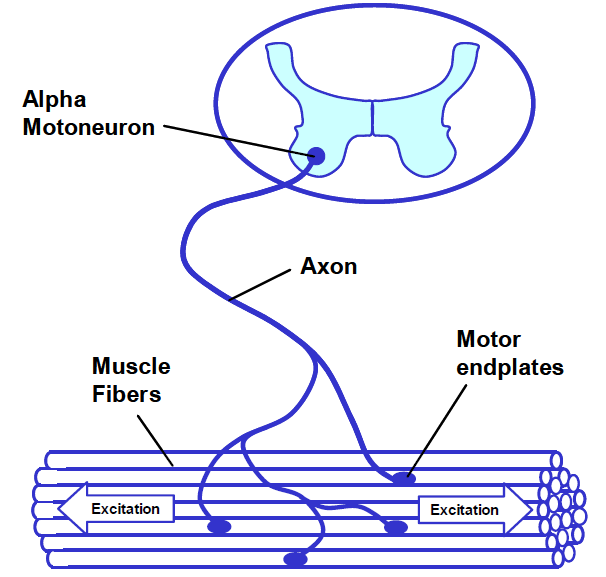
\includegraphics[width=0.4\textwidth]{figures/Anatomy/EMG_generation}  %<--but is not needed.
	\caption{Illustration of the action potential exciting the muscle fibre, which causes the release of calcium ions and the muscle to contract. \cite{konrad2005}}
	\label{fig:EMG_generation}  %<--give the figure a label, so you can reference!
\end{figure}


The muscle fibre is an excitable cell with a resting potential of between -90mV and -70mV. A threshold of approximately -55mV needs to be reached for an action potential to be generated, this is visualised in \figref{fig:action_potential}. The sarcolemma, the membrane covering the muscle fibres, has sodium and potassium ion channels that maintains the resting potential, depolarize the muscle fibre if the threshold is exceeded or repolarize the muscle fibre. \cite{cram2012}


\begin{figure}[H]
	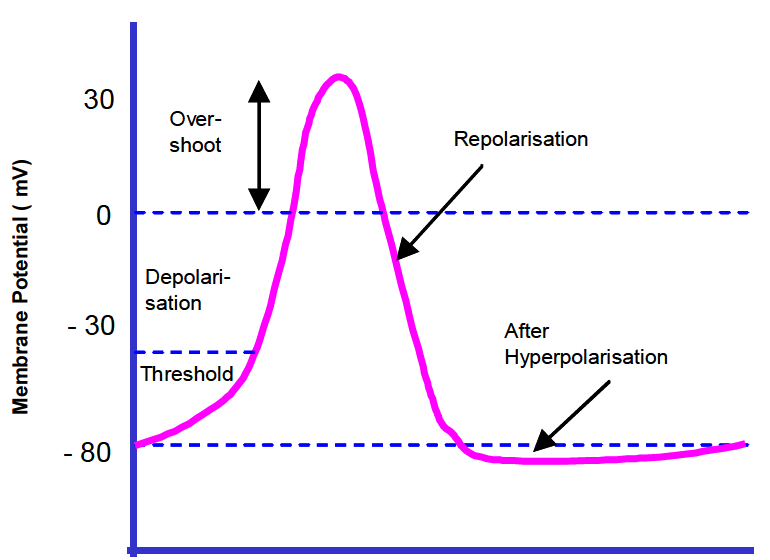
\includegraphics[width=0.5\textwidth]{figures/Anatomy/action_potential}  %<--but is not needed.
	\caption{Illustration of the action potential exceeding the threshold for it to be generated and the following depolarization and repolarization. \cite{konrad2005}}
	\label{fig:action_potential}  %<--give the figure a label, so you can reference!
\end{figure}

The lower motor axon is branching out so that it can attach to the muscle fibre at the motor end-plate and create neuromuscular synapses. 

The action potential travelling down the axon reaches the synapses and releases Acetylcholine (ACh). ACh raises the permeability of the cell membrane where sodium ions influx and causes the membrane to depolarize. 
This creates a new action potential that travels along the whole muscle fibre along the sarcolemma.
% and through t-tubules to reach the sarcoplasmatic reticulum inside the muscle. The sarcoplasmatic reticulum encapsulates the muscle fibres and release calcium ions which binds with troponin and expose the active sites on the thin filaments in the muscle fibres which allows the muscle to contract, when the myocin heads 
This happens in both directions from the motor end-plate to the tendinous attachment. When the peak of the depolarization of about 30mV is reached a rapid efflux of potassium ions causes the muscle fibre to repolarize and reach its resting potential again. This is the action potential which is recorded with EMG. \cite{cram2012}

Depending on the force that needs to be applied for a given task more or less motor units are activated and therefore more or less muscle fibres are contracted. The bigger the force the more motor units are activated. Furthermore, the number of muscle fibres per motor unit varies between muscles in the human anatomy. The finer the movement the higher the innervation, e.g. the lower arm muscles have a higher innervation than those in the quadriceps. \cite{cram2012}

\subsection{Recording of electromyography}

Recording of EMG can be done either at the skin surface (sEMG) or intra muscular (iEMG). sEMG is performed using electrodes placed on the skin while iEMG is done using needle electrodes inserted into the muscle, but sEMG is far more commonly used as it is non-invasive and easy to use. \cite{cram2012}  

When acquiring sEMG signals the electrodes act as a transducer by converting the recorded action potentials from the muscles into an electric current. Surface electrodes used to acquire EMG signals comes both with and without gel covered surfaces, where the use of dry electrodes will often be more practical in use, while the gel covered electrodes will acquire more exact readings of the signals. \cite{lee2008, cram2012}

%where the the Myo armband employs dry electrodes.
The most commonly used electrodes for EMG are made of disposable silver-impregnated plastic, and in order to keep the electric potential on the skin surface stable and reduce impedance between the surfaces, they are often covered in a silver chloride gel. Using dry electrodes will result in a higher surface impedance, which means that the signal contains more noise compared to a gel covered electrode. However, when using dry electrodes the skin will itself provide a “gel” by sweating which will decrease the skin impedance. \cite{cram2012}

%the extraocular muscle has the highest innervation of 3:1 and the gastrocnemius muscles has one of 2000:1. \cite{cram2012}

%(Something about how the innervation is in certain muscles of the forearm. Also argue that humans can perform more dexterous movement when the ratio of muscle fibers to motor units is low) (maybe around 100:1)

%(something about how the EMG signal is affected when the limb is positioned differently)
% following section move to the "conclusion of the background" section
%As mentioned this project focuses on the mapping of different hand gestures. This mapping relies on that the generated EMG from the different hand gestures are differentiable. For a prosthetic user a good performing prosthesis must perform hand gestures as well in an elevated limb position as in a seated position to be able to support the user in daily tasks, e. g. taking a cup from a cupboard and pouring water into the cup. However, changes in the EMG occurs when performing the same hand gestures in different limb positions. These signal alternations can occur for different reasons. Changing the limb position can lengthen the muscles and result in a change in the signal source relative to the electrode from which the EMG signal is obtained, and even the lengthening of the muscles itself due to changing limb position will alter the EMG activity caused by a degree of overlap of the thick and thin filaments. Other findings has shown that the activity of certain muscles' is depending on angles of joints besides those primarily actuating the contraction of these muscles. \cite{Fougner2011} Thus, this limb position effect must be seen as an important aspect to take into consideration in the mapping of hand gestures to control a prosthesis for the user to receive a good performing support device. 